\documentclass[11pt]{article}
\usepackage[english]{babel}
\usepackage{geometry}
\usepackage{amsmath}
\usepackage{amsthm}
\usepackage{graphicx}
\usepackage[utf8]{inputenc}

%%%%%%%% MARGIN
\geometry{verbose, letterpaper, tmargin=3cm,
  bmargin=3cm,lmargin=2.5cm,rmargin=2.5cm}

%%%%%%%% NO PARAGRAPH INDENT
% https://tex.stackexchange.com/questions/27802/set-noindent-for-entire-file
\setlength\parindent{0pt}

%%%%%%%% SUB-FIGURE PACKAGE
\usepackage{subcaption}

%%%%%%%% HYPERREF PACKAGE
\usepackage{hyperref}
\hypersetup{linkcolor=blue}
\hypersetup{citecolor=blue}
\hypersetup{urlcolor=blue}
\hypersetup{colorlinks=true}

%%%%%%%% DEFINITION AND THEOREM DEFINITIONS
\theoremstyle{definition}
\newtheorem{definition}{Definition}[section]

\theoremstyle{remark}
\newtheorem{remark}{Remark}

\theoremstyle{remark}
\newtheorem{question}{Question}

\newtheorem{theorem}{Theorem}[section]

%%%%%%%% MULTI-COLUMNS PACKAGE
\usepackage{multicol}

%%%%%%%% BIB-LATEX STUFF
\usepackage[style=numeric,
            bibstyle=numeric,
            citestyle=numeric,
            hyperref=true,
            backend=biber]{biblatex}
\addbibresource{ref.bib} %Put relative path to ref

%%%%%%%% SETS DEFINITIONS
\usepackage{amssymb}
%%%% Important sets
\renewcommand{\O}{\mathbb{O}}
\newcommand{\N}{\mathbb{N}}
\newcommand{\Z}{{\mathbb{Z}}}
\newcommand{\Q}{{\mathbb{Q}}}
\newcommand{\R}{{\mathbb{R}}}

%%%% Statistics
\newcommand{\E}[1]{\mathbb{E}\left[#1 \right]}
\newcommand{\V}[1]{\mathrm{Var}\left[#1 \right]}

%%%% Lambda Calculus Symbols
\newcommand{\dneq}{\,\, \# \,\,}
\renewcommand{\S}{\pmb{\mathrm{S}}}
\newcommand{\I}{\pmb{\mathrm{I}}}
\newcommand{\K}{\pmb{\mathrm{K}}}
\newcommand{\ch}[1]{\ulcorner #1 \urcorner}

%%%% Ordinal Lambda Calculus Symbols
\newcommand{\ordAlph}{\Sigma_{\text{Ord}}}
\newcommand{\termOrd}{\text{Term}_\text{Ord}}
\newcommand{\fl}{\mathrm{fl}}
\newcommand{\sk}{\mathrm{sk}}

%%%% Superscript to the left
% https://latex.org/forum/viewtopic.php?t=455
\usepackage{tensor}
\newcommand{\app}[3]{\tensor*[^{#1}]{\left(#2, #3\right)}{}}

%%%% Make optional parameter
% https://tex.stackexchange.com/questions/217757/special-behavior-if-optional-argument-is-not-passed
\usepackage{xparse}
\NewDocumentCommand{\cx}{o}{
  \IfNoValueTF{#1}
  {\left[\quad\right]}
  {\left[\, #1 \,\right]}
}

%%%%%%%% LOGIC TREES
\usepackage{prftree}

%%%%%%%% SPLIT EQUATIONS
% https://tex.stackexchange.com/questions/51682/is-it-possible-to-pagebreak-aligned-equations
\allowdisplaybreaks

%%%%%%%% FLOAT SPECIFIER
% https://www.overleaf.com/learn/latex/Errors/LaTeX_Error:_Unknown_float_option_%60H%27
\usepackage{float}

%%%%%%%% CODE RENDERING !!! UNCOMMENT IF NEEDED !!!
% Compile with flag -shell-escape
%\usepackage{minted}

%%%%%%%% START DOCUMENT

\title{Non-Parametric Statistics Workshop 1}
\author{David Plazas Escudero \\
  Juan Pablo Vidal \\
  Juan Sebasti\'an C\'ardenas-Rodríguez \\
  \scalebox{0.7}{Mathematical Engineering, Universidad EAFIT}}
\date{\today}


\begin{document}
\maketitle
\section{Workshop Exercises}
\subsection*{Exercise 3}
Calculate and plot the confidence bands for the empirical continuous
distribution function (ECDF) of the coldest and hottest year in
average with a confidence of 95 \% . Are there any sectors that are
not enclosed in the bands?

\begin{proof}
  Let $n$ be the size of the sample and $1 - \alpha$ the desired
  confidence for the bands. To calculate the confidence bands for the
  ECDF, we first define $\epsilon_n$ by the following formula:
  \begin{equation*}
    \epsilon_n = \sqrt{\frac{1}{2n} \ln\left(\frac{2}{\alpha}\right)}
  \end{equation*}

  Let $\hat{F}_n(x)$ be the ECDF. Then, for each $x$ in the ECDF we
  define the lower ($L(\cdot)$) and upper ($U(\cdot)$) bound by:
  \begin{align*}
    L(x) &= \max\{\hat{F}_n(x) - \epsilon_n, 0\} \\
    U(x) &= \min\{\hat{F}_n(x) + \epsilon_n, 1\}
  \end{align*}

  The results obtained by using the temperatures of the coldest and
  hottest year are seen in Figure \ref{fig:ex3}.
  \begin{figure}[H]
    \centering
    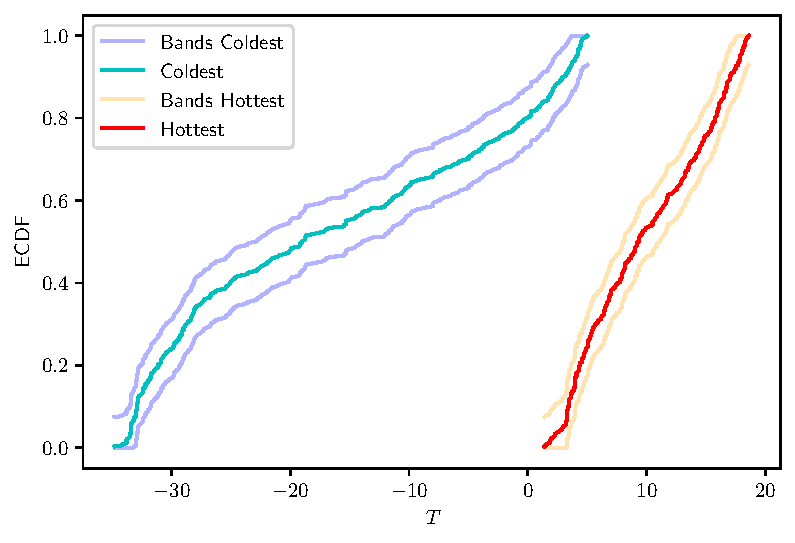
\includegraphics[scale=0.5]{../figs/ecdf_bands.pdf}
    \caption{Bands for the coldest and hottest year.}
    \label{fig:ex3}
  \end{figure}

  It can be seen that the upper and lower bands fully enclose the
  ECDF. Nevertheless, there exists two points where the function and
  the bands meets. This happens in the lower band at the beginning and
  the upper band at the final point.

  This phenomenon is due to the full certainty at those points in a
  sense that the lower bound, at the start, has to be the same point
  as it cannot go lower than 0. A similar reasoning can explain the
  upper bound and the final point.
\end{proof}

\subsection*{Exercise 4}

\subsection*{Exercise 7}

\subsection*{Exercise 11}

\subsection*{Exercise 12}

\subsection*{Exercise 14}

\section{Book Exercises}
All exercises in this section are extracted from \parencite{wasserman2006}.

\subsection*{Exercise 16--10}

\printbibliography
\end{document}
